\documentclass[11pt,a4paper]{article}
\usepackage[utf8]{inputenc}
\usepackage[T1]{fontenc}
\usepackage[margin=2.5cm]{geometry}
\usepackage{amsmath,amssymb}
\usepackage{graphicx}
\usepackage{booktabs}
\usepackage{siunitx}
\usepackage{microtype}
\usepackage{float}
\usepackage{xcolor}
\usepackage[font=small,labelfont=bf]{caption}
\usepackage[authoryear,round]{natbib}
\usepackage[colorlinks=true,linkcolor=blue!50!black,citecolor=blue!50!black,urlcolor=blue!50!black]{hyperref}
\usepackage[capitalise,noabbrev]{cleveref}

\graphicspath{{../figures/}}

\title{Sorting Board Games with a Pick-and-Place Robot:\\ an Exact Benchmark, and What the Model Leaves Out}
\author{Juan Carlos Chavarr\'ia Morales\\[2pt]
  \small M.Sc.\ Optimization, Hochschule Bielefeld (HSBI)\\
  \small Course \emph{Discrete Simulation and Reinforcement Learning}, summer term 2026}
\date{October 2026}

\begin{document}
\maketitle

\begin{abstract}
In a Plant Simulation model of a board-game factory, games in three languages reach a pick-and-place robot in
random order. The robot puts each game into one of two intermediate storages or sends it around a conveyor loop;
a storage takes one language only, a game of another language sends its partial batch back to the loop, and ten
equal games leave the storage as a batch. A reinforcement-learning agent is to control the robot so that 1000
games are finished as quickly as possible. We formulate the decision problem as a stochastic shortest-path problem
(163\,923 states), solve it exactly by value iteration and use the solution to validate tabular Q-learning: the
learned policy is within \SI{0.06}{\percent} of the optimum, and both are \SI{14}{\percent} cheaper than the greedy
heuristic used as baseline in the course, mostly by evicting small batches where the heuristic loops. The model,
however, treats looped and evicted games as gone, while in the plant they return to the robot. On a decision-level
model of the plant that lets them return, the ``optimal'' policy needs up to a third more robot decisions than
the greedy heuristic, and with a loop that has priority at the merge both policies can lock the
robot in an endless loop. Q-learning on the plant model, started from the model's solution, is the only policy
that beats the heuristic there (\SI{1.8}{\percent} fewer decisions, \SI{40}{\percent} less spread). The repository
contains the SimTalk methods and the COM client that connect the agent to the Plant Simulation model.
\end{abstract}

% =====================================================================================================================
\section{The plant and the decision}

The Plant Simulation model \citep{Bangsow2020} produces board games in three language variants. Manual sheets
(language-specific, unsorted) are bound in a binding station, game material is painted, and an assembly station
combines one manual and one set of material into a game; the manual is the main part, so the game carries the
language of its manual (\texttt{DE}, \texttt{EN}, \texttt{ES}) as its name. The finished games run unsorted on one
conveyor into the warehouse complex, where the pick-and-place robot decides for each game:

\begin{itemize}
  \item \texttt{A}: into intermediate storage \texttt{bufferID1}; \texttt{B}: into \texttt{bufferID2};
  \item \texttt{LOOP}: back to the entrance of the complex via the loop \texttt{Return\_to\_mainCon}.
\end{itemize}
A storage holds games of one language only. Placing a game of another language sends all games already in the
storage back to the entrance through the loop (an \emph{eviction}). When a storage holds ten equal games, it is
emptied into the sink. The objective of the project is to minimise the throughput time of 1000 games.

\paragraph{Parameters.} The repository takes its identities and parameters from the Plant Simulation model
(\texttt{plantsim/}): the language shares of the source table \texttt{SystemLoad} (DE 0.40, EN 0.35, ES 0.25), the
storage capacity and batch size 10, the goal of 1000 games (variable \texttt{GoalGames}), and the action strings
\texttt{A}, \texttt{B}, \texttt{LOOP} written by the agent into the table \texttt{ActionControl}. The course
exercise on language variants used shares 0.2/0.5/0.3 and a first formulation 0.4/0.3/0.3; \cref{sec:shares}
shows how much the shares matter.

% =====================================================================================================================
\section{The decision problem as a stochastic shortest path}

\paragraph{State and actions.} At a decision the robot holds a game of language $\lambda \in \{1,2,3\}$. Storage
$i \in \{1,2\}$ holds $n_i \in \{0,\dots,9\}$ games of language $q_i \in \{0,1,2,3\}$ ($q_i = 0$: empty; a tenth game
triggers the flush, so ten are never stored), and $k \in \{0,\dots,100\}$ batches have been completed. The state is
$s = (q_1, n_1, q_2, n_2, \lambda, k)$; with the consistency constraints ($n_i = 0 \Leftrightarrow q_i = 0$, the two
storages never hold the same language) there are 163\,923 states, of which those with $k = 100$ are terminal. The
actions are \texttt{A}, \texttt{B} and \texttt{LOOP}; placing a game into the storage that holds the other storage's
language is infeasible.

\paragraph{Transitions.} An action changes the storage contents deterministically (placement, eviction, flush with
$k \to k+1$); the next game at the robot is a new draw with the language shares $p = (0.40, 0.35, 0.25)$. This is the
central simplification: a looped or evicted game does not come back, it is replaced by a fresh game from the
source.

\paragraph{Costs.} Every decision costs $c_\text{route} = 1$; a loop costs $c_\text{loop} = 2$ more, an eviction
$C_\text{lin} = 1.5$ per evicted game:
\begin{equation}
  c(s,a) = c_\text{route} + c_\text{loop}\,\mathbf 1[a = \texttt{LOOP}]
         + C_\text{lin}\, n_i\, \mathbf 1[a \text{ evicts storage } i].
\end{equation}
Every decision costs time, a loop costs the time of a round trip, and an eviction the round trips of the evicted
games, so the total cost is a proxy of the throughput time.

\paragraph{Why a stochastic shortest path.} An episode ends when the goal $k = 100$ is reached, not after a fixed
number of steps, and every policy that keeps placing games eventually reaches it. The problem is a stochastic
shortest-path problem \citep{Bertsekas1991}: all costs are positive, improper policies (those that loop forever)
have infinite cost, so the undiscounted Bellman equation
\begin{equation}
  V^*(s) = \min_{a \in A(s)} \Big[c(s,a) + \sum_{\lambda'} p_{\lambda'}\, V^*\big(f(s,a,\lambda')\big)\Big],
  \qquad V^*(s) = 0 \text{ for } k = 100,
\end{equation}
has a unique solution and $\gamma = 1$ is the correct choice: the objective is the total cost of the episode.

% =====================================================================================================================
\section{Exact solution and benchmark}

\paragraph{Value iteration.} The counter $k$ never decreases and a transition changes it by at most one, so the
problem decomposes into 100 layers of about 1\,600 states each, solved backwards from $k = 99$; the layered solution
agrees with plain value iteration over the full space. The optimal expected cost from an empty warehouse is
$V^* = 1965.0$; the greedy heuristic of the course (put a game into the storage that holds its language, else into
an empty storage, else loop; never evict) costs $2288.7$, \SI{16.5}{\percent} more (\cref{tab:benchmark}). The
optimal policy differs from the heuristic in one kind of decision: where the heuristic loops a game because both
storages hold other languages, the optimal policy evicts a small partial batch. In simulation the optimal policy
needs 1334 robot decisions for 1000 games, the heuristic 1433, with 276 against 429 loops.

\begin{table}[t]
  \centering\small
  \caption{Exact expected cost, simulated cost (1000 episodes), robot decisions, loops and evictions for 1000
    games, on the SSP model.}
  \label{tab:benchmark}
  \begin{tabular}{lrrrrr}
\toprule
policy & exact $J$ & simulated cost & decisions & loops & evictions \\
\midrule
optimal (value iteration) & 1965.0 & 1965.8 $\pm$ 62.2 & 1334 & 276 & 35.2 \\
Q-learning & 1966.1 & 1965.2 $\pm$ 62.1 & 1334 & 275 & 37.0 \\
greedy baseline & 2288.7 & 2290.5 $\pm$ 88.6 & 1433 & 429 & 0.0 \\
\bottomrule
\end{tabular}

\end{table}

\paragraph{Q-learning.} Tabular Q-learning \citep{Sutton2018} with 512 parallel environments, count-based step sizes
and $\varepsilon$-greedy exploration learns in 31 seconds (5000 episodes) a policy with expected cost $1966.1$,
\SI{0.06}{\percent} above the optimum; it agrees with the optimal policy in \SI{98.5}{\percent} of all states and
\SI{99.0}{\percent} of those the optimal policy visits (\cref{fig:benchmark}). The agent learns over the storage
configuration without $k$, with $\gamma = 0.99$, which makes the table a hundred times smaller. The exact
decomposition of its gap, each term evaluated exactly on the undiscounted problem, is \num{0.65} from discounting,
\num{0.18} from ignoring $k$ and \num{0.30} from learning; the price of discounting falls from \SI{2.4}{\percent} at
$\gamma = 0.9$ to \SI{0.003}{\percent} at $\gamma = 0.999$ (\cref{fig:gamma}).

\begin{figure}[t]
  \centering
  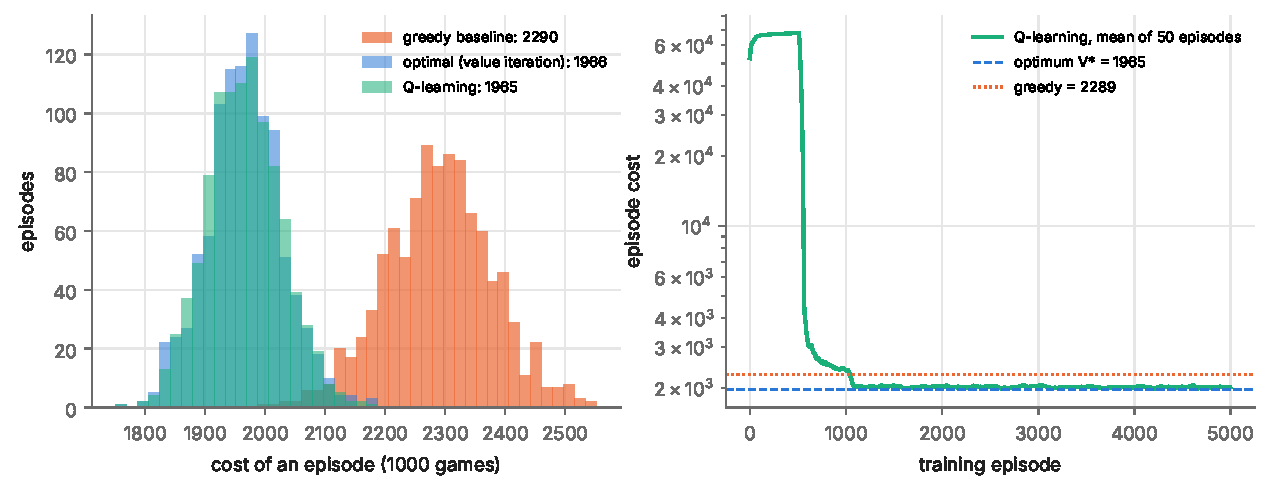
\includegraphics[width=\linewidth]{benchmark.pdf}
  \caption{Left: cost of 1000 simulated episodes for the three policies. Right: training of Q-learning.}
  \label{fig:benchmark}
\end{figure}

\begin{figure}[t]
  \centering
  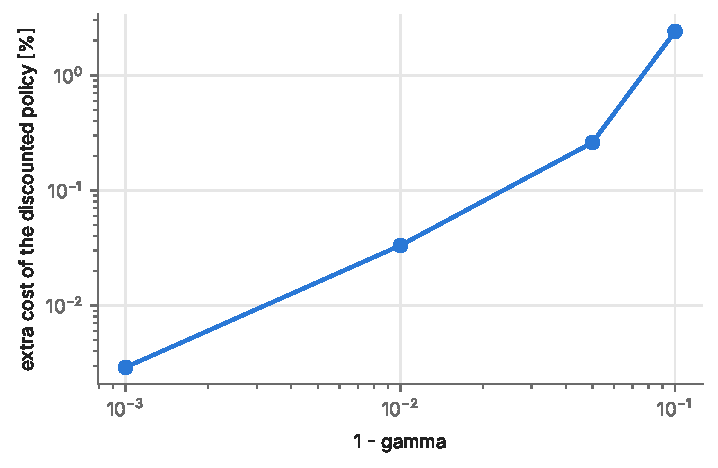
\includegraphics[width=0.5\linewidth]{gamma.pdf}
  \caption{Extra cost on the undiscounted problem of the policy that is optimal for discount factor $\gamma$.}
  \label{fig:gamma}
\end{figure}

\paragraph{Language shares.}\label{sec:shares} The more unequal the shares, the more there is to gain over the
heuristic (\cref{tab:shares}): \SI{24}{\percent} with the shares of the course exercise (0.2/0.5/0.3), \SI{14}{\percent}
with those of the plant model, \SI{2}{\percent} with equal shares. With equal shares no language is rare enough for an
eviction to pay off.

\begin{table}[H]
  \centering\small
  \caption{Optimum and greedy heuristic for different language shares.}
  \label{tab:shares}
  \begin{tabular}{lrrr}
\toprule
shares DE/EN/ES & optimum $V^*$ & greedy & saving \\
\midrule
course task 4 (0.2/0.5/0.3) & 1731 & 2287 & 24.3\% \\
first formulation (0.4/0.3/0.3) & 2133 & 2289 & 6.8\% \\
Plant Simulation model (0.4/0.35/0.25) & 1965 & 2289 & 14.1\% \\
equal (1/3 each) & 2244 & 2289 & 2.0\% \\
\bottomrule
\end{tabular}

\end{table}

% =====================================================================================================================
\section{Connecting the agent to Plant Simulation}

The environment has two backends with the same interface and the same state encoding: the SSP of the previous
sections, and the Plant Simulation model through its COM interface. In the model (\texttt{plantsim/methods}), the
exit control \texttt{pnpDecision} of the robot fires when a game is ready to leave it, writes the state into the table
\texttt{CurrentState} (language of the game, contents of both storages, games in the loop, finished batches,
simulated time), increments an event counter and stops the event controller. The Python client waits for the new
event, writes \texttt{A}, \texttt{B} or \texttt{LOOP} into \texttt{ActionControl} and runs \texttt{AIControl}, which
applies the action with the rules of the SSP (eviction to the loop, flush of ten equal games to the sink), records
loop, eviction and batch flags for the cost, and restarts the simulation until the next game reaches the robot.
\texttt{reset} sets the random seed and runs the model to the first decision. The protocol is tested against a mock
of the model; the repository has not been run against a live Plant Simulation licence.

% =====================================================================================================================
\section{What the model leaves out: games come back}

In the plant, a looped or evicted game is not replaced by a new one: it travels around the loop and reaches the robot
again. The mock of the model reproduces this at the level of decisions: a game sent around returns $d$ decisions
later. Where the loop joins the main conveyor, returning games and new games from the source are merged, either in
turn (\emph{alternate}) or with priority for the loop (\emph{loop first}).

\begin{table}[t]
  \centering\small
  \caption{Robot decisions for 1000 games (mean of 30 episodes; at most 6000 decisions) when looped and evicted games
    return after $d$ decisions.}
  \label{tab:recirculation}
  \begin{tabular}{llrr}
\toprule
games return after & merge & MDP optimum & greedy \\
\midrule
never (MDP) & - & 1335 & 1436 \\
5 & alternate & 1989 & 1768 \\
20 & alternate & 1932 & 1454 \\
60 & alternate & 1903 & 1436 \\
5 & loop first & --- (none finished) & --- (none finished) \\
20 & loop first & 1724 (11/30 finished) & 1500 (12/30 finished) \\
60 & loop first & 1772 & 1428 \\
\bottomrule
\end{tabular}

\end{table}

\begin{figure}[t]
  \centering
  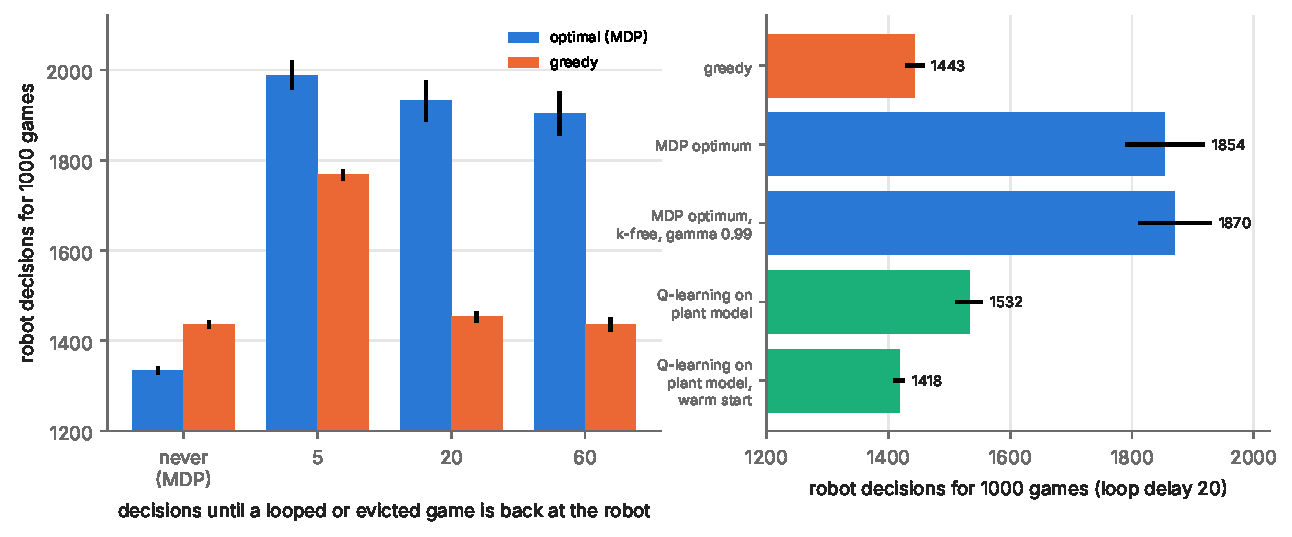
\includegraphics[width=\linewidth]{recirculation.pdf}
  \caption{Left: decisions for 1000 games when games return (alternate merge; 95\% confidence intervals). Right:
    policies on the plant model with $d = 20$, including Q-learning trained on it.}
  \label{fig:recirculation}
\end{figure}

\Cref{tab:recirculation,fig:recirculation} show the consequence. As soon as games return, the policy that is optimal
for the SSP is the worst of the two: it needs about 1900--2000 decisions against 1440--1770 for the heuristic. Its
advantage came from evictions and loops whose games were assumed to vanish; in the plant every evicted game costs
another decision later, and an eviction sends up to nine games around at once. The heuristic, which never evicts,
is almost unaffected when games take long to return. The merge rule matters as much: when returning games have
priority and return quickly, the robot sees only returning games once as many games circulate as decisions fit in
one round trip, the source is starved and the episode never ends, for both policies. In the plant this is a
property of the conveyor layout to check before any training.

\paragraph{Learning on the plant model.} Q-learning on the plant model ($d = 20$, alternate merge; 1500 episodes,
state without $k$, $\gamma = 0.99$; the contents of the loop are not observed) gives the results of
\cref{tab:plant}. From scratch it does not reach the heuristic (1533 decisions); started from the solution of the
SSP, it corrects the model's mistakes and finishes 1000 games in 1418 decisions, \SI{1.8}{\percent} fewer than the
heuristic and with \SI{40}{\percent} less spread. It still evicts, but with fewer loops.

\begin{table}[H]
  \centering\small
  \caption{Policies on the plant model with returning games ($d = 20$, alternate merge; 30 episodes, mean $\pm$
    standard deviation).}
  \label{tab:plant}
  \begin{tabular}{lrrr}
\toprule
policy & decisions for 1000 games & loops & evictions \\
\midrule
greedy & 1443 $\pm$ 44 & 438 & 0 \\
optimal MDP policy (gamma = 1) & 1854 $\pm$ 182 & 761 & 51 \\
k-free discounted MDP policy (warm-start point) & 1870 $\pm$ 167 & 769 & 58 \\
Q-learning on the plant model, from scratch & 1532 $\pm$ 64 & 424 & 83 \\
Q-learning on the plant model, warm start & 1418 $\pm$ 26 & 332 & 76 \\
\bottomrule
\end{tabular}

\end{table}

% =====================================================================================================================
\section{Main changes with respect to the original benchmark}

\begin{table}[H]
  \centering\small
  \caption{Main changes with respect to the benchmark written during the course.}
  \label{tab:changes}
  \begin{tabular}{p{0.2\linewidth}p{0.34\linewidth}p{0.38\linewidth}}
    \toprule
    & course benchmark & this version \\
    \midrule
    Identities & languages L1--L3, storages S1/S2, action \emph{loop} & DE/EN/ES, \texttt{bufferID1}/\texttt{bufferID2}
      (\texttt{A}/\texttt{B}), \texttt{LOOP} = \texttt{Return\_to\_mainCon}, as in the Plant Simulation model \\
    Parameters & shares 0.4/0.3/0.3 (report), 0.4/0.35/0.25 (code) & 0.4/0.35/0.25 from \texttt{SystemLoad};
      sensitivity to the shares of the course exercise \\
    Plant interface & socket backend announced, not implemented & SimTalk methods and COM client following one
      decision protocol; mock of the model for tests \\
    Validation & optimum, Q-learning, $\gamma$ sweep on the SSP & in addition: returning games, merge rules,
      Q-learning on the plant model \\
    Code & scripts in one folder & package, scripts for every result, tests \\
    \bottomrule
  \end{tabular}
\end{table}

% =====================================================================================================================
\section{Conclusions}

\begin{enumerate}
  \item As a stochastic shortest-path problem the sorting task is small enough to be solved exactly; the optimum is
    \SI{14}{\percent} cheaper than the greedy heuristic, mainly by evicting small batches instead of looping.
  \item Tabular Q-learning reaches the optimum within \SI{0.06}{\percent}; the exact decomposition of its gap shows
    that discounting, not learning, is its largest part.
  \item The SSP assumes that looped and evicted games vanish. In the plant they return, and then the policy that is
    optimal for the SSP needs up to a third more robot decisions than the heuristic. The benchmark validates the learning
    algorithm, not the model of the plant.
  \item Learning on a model with returning games, started from the SSP solution, beats the heuristic, but by
    \SI{2}{\percent}, not \SI{14}{\percent}. The merge of the loop into the main conveyor must be checked first: with
    priority for the loop the robot can be starved of new games.
  \item The next steps are training on the Plant Simulation model itself through the COM interface, with the simulated
    time as cost, and a state that includes the games in the loop.
\end{enumerate}

\section*{Code}
Code, SimTalk methods and the scripts for every number of this report: \citet{Repo}.

\bibliographystyle{plainnat}
\bibliography{references}

\end{document}
